%!TEX root =  DICA.tex
\onecolumn
\appendix

\section{Experimental Results for dimension 3}
\label{sec:results_d3}
We report the reconstruction errors for different kinds of mixing matrices (dimension 3) and noise ratios.

\begin{figure}[t] %pt]
	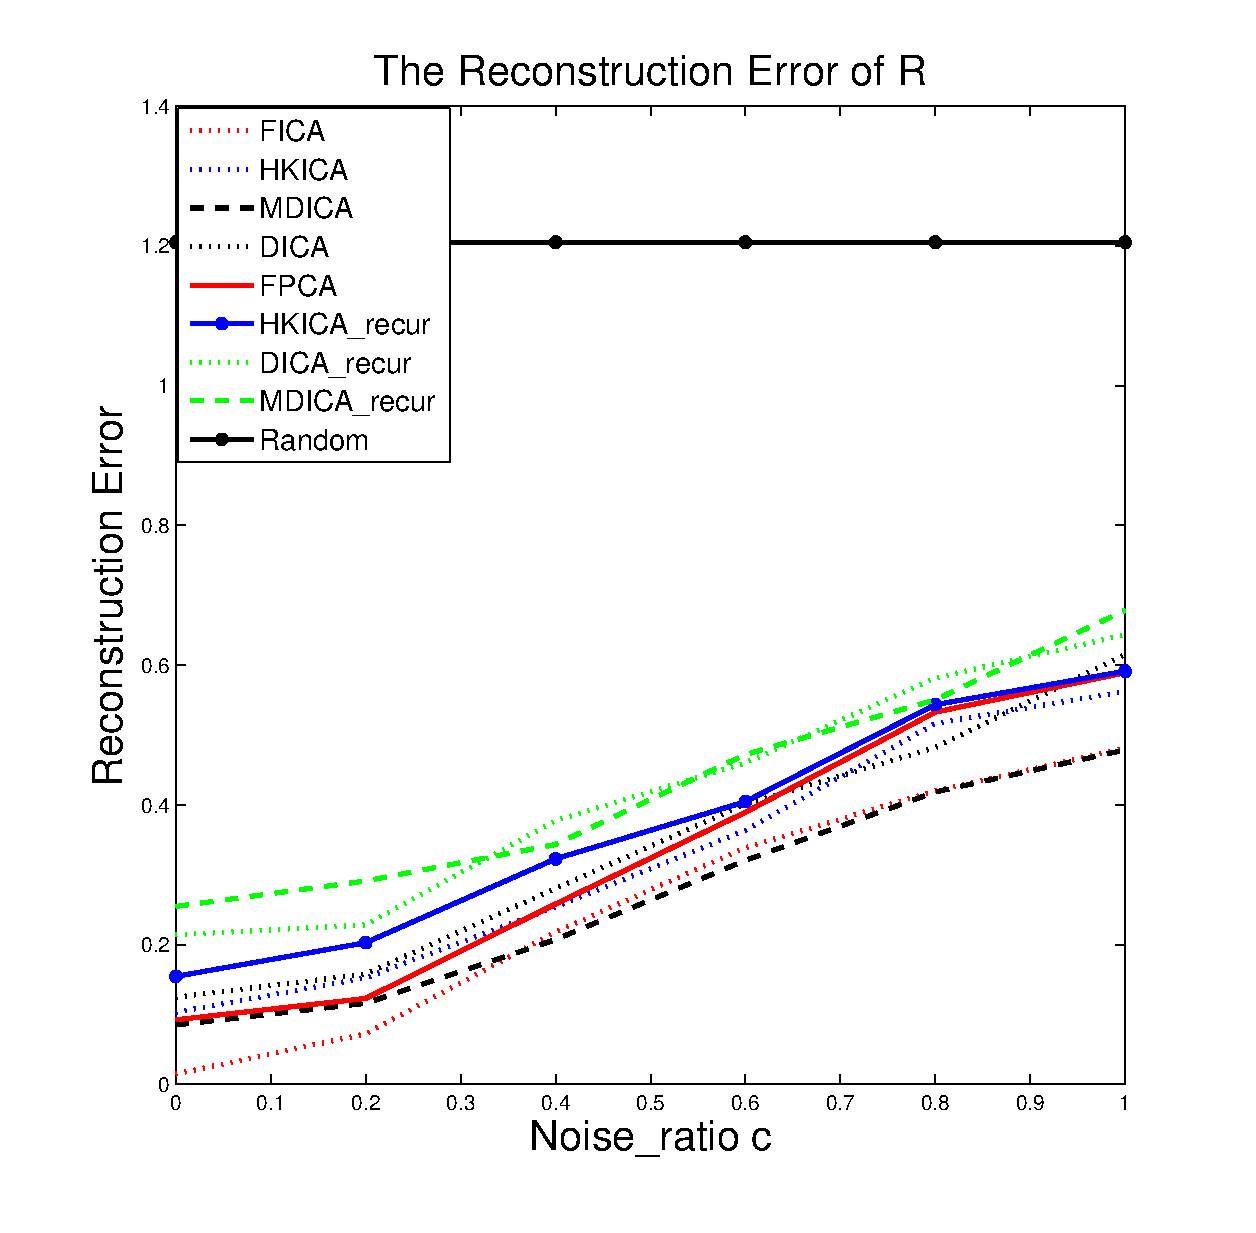
\includegraphics[width =0.45\columnwidth]{errorR_d3}
	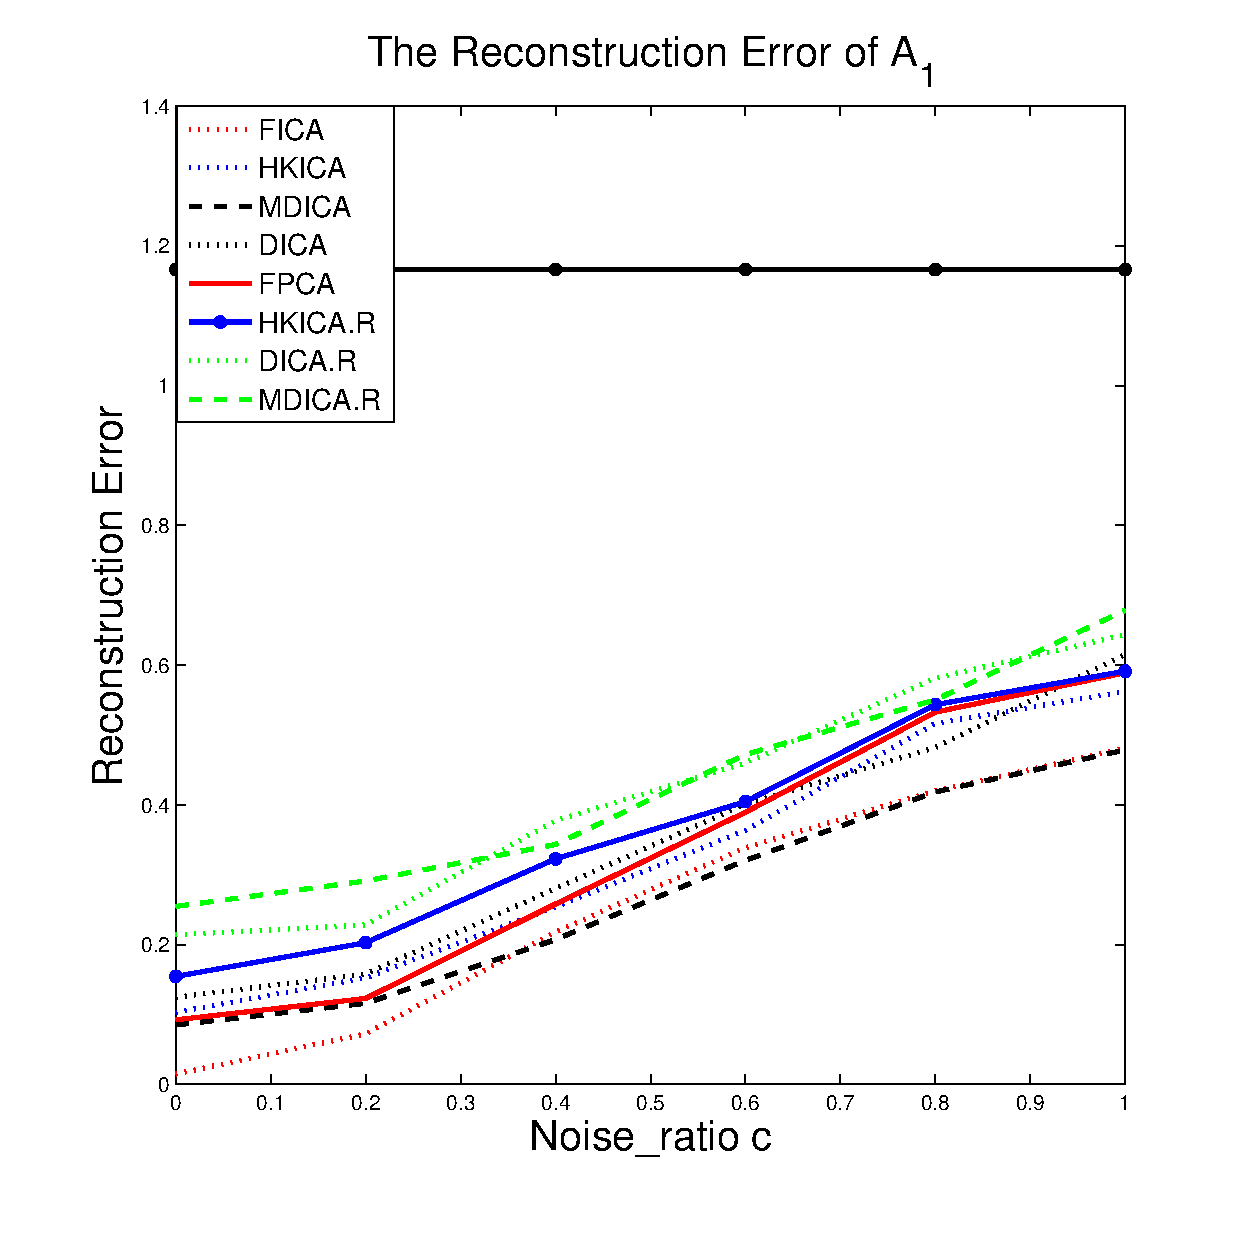
\includegraphics[width =0.45\columnwidth]{error1_d3} \\
	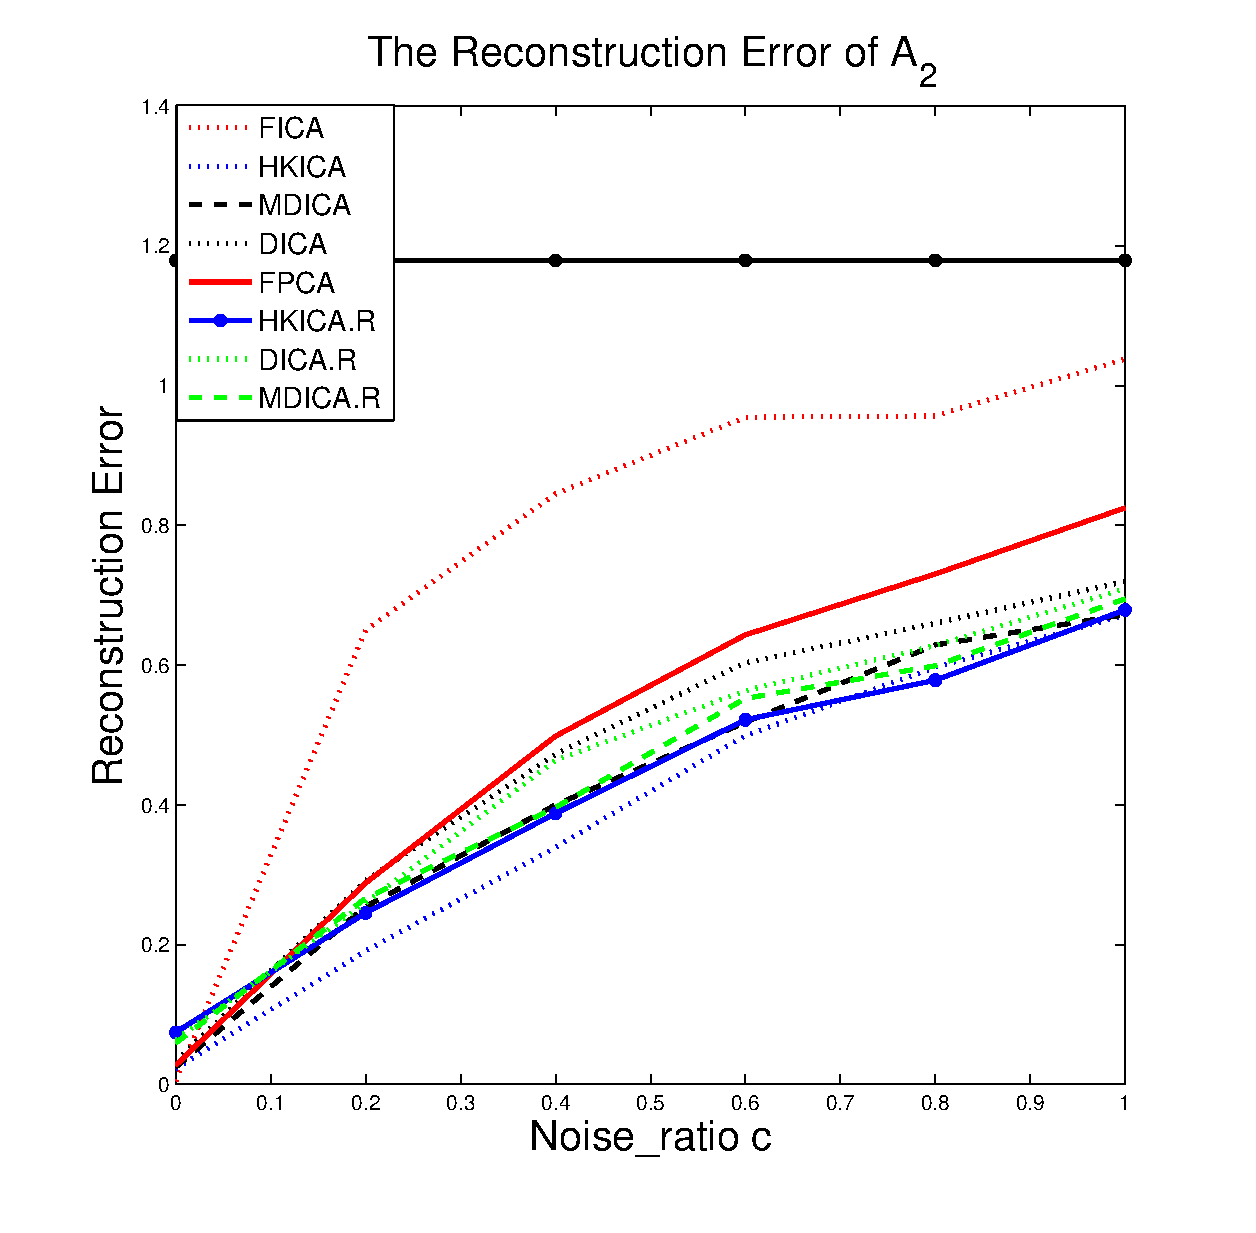
\includegraphics[width =0.45\columnwidth]{error2_d3}
	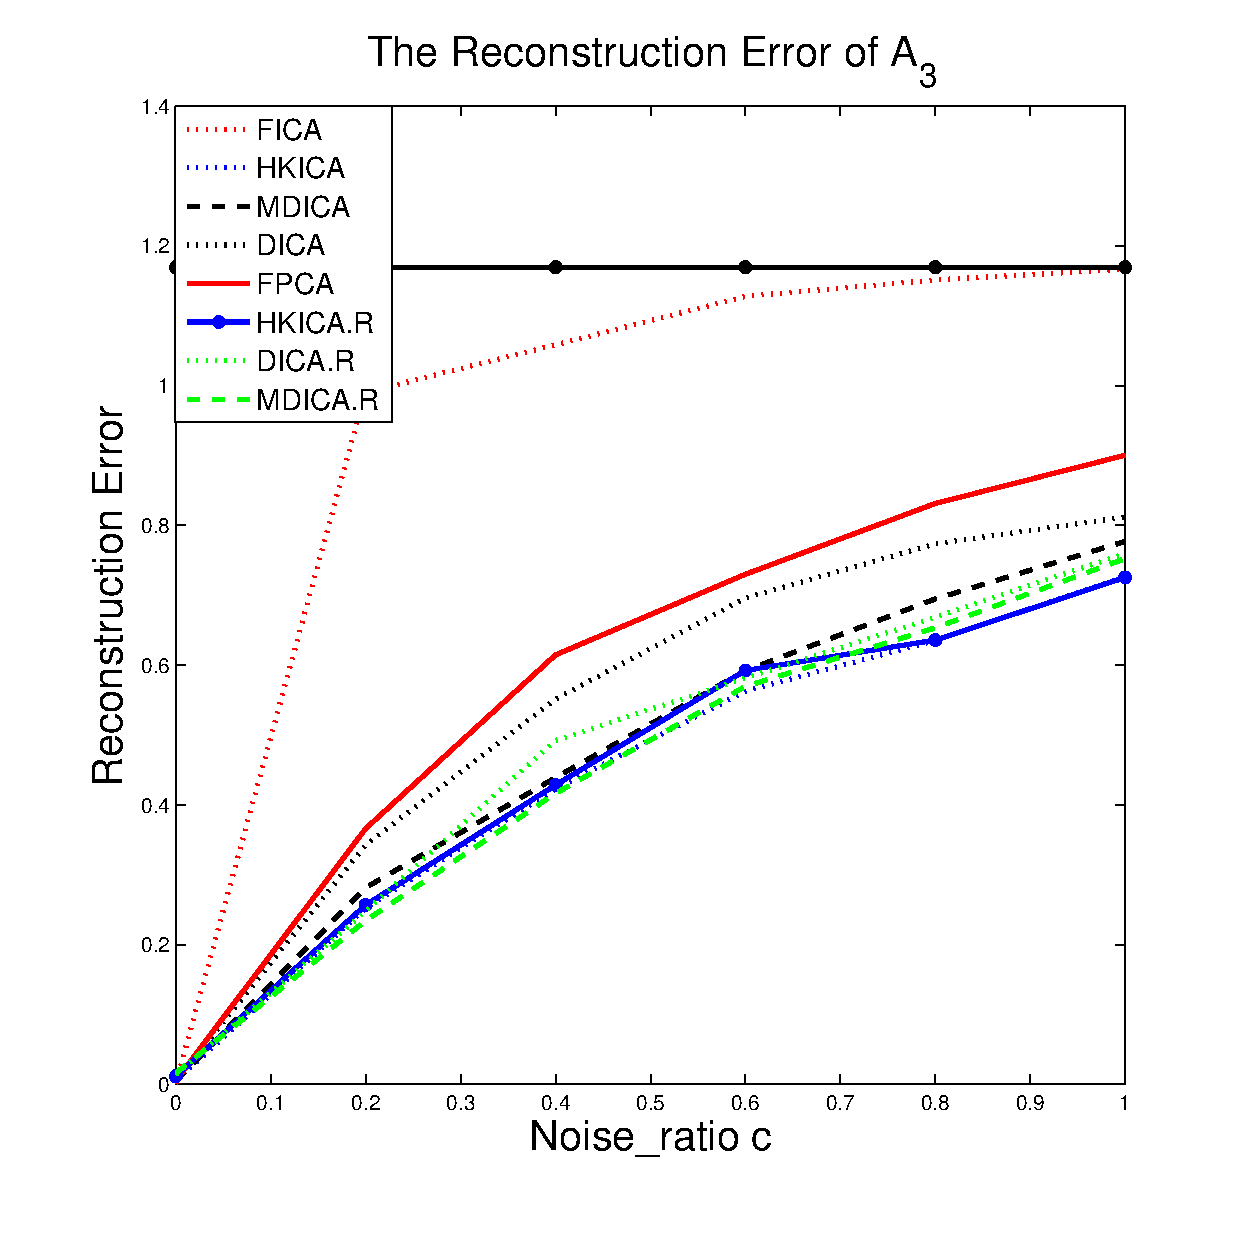
\includegraphics[width =0.45\columnwidth]{error3_d3}  \\
	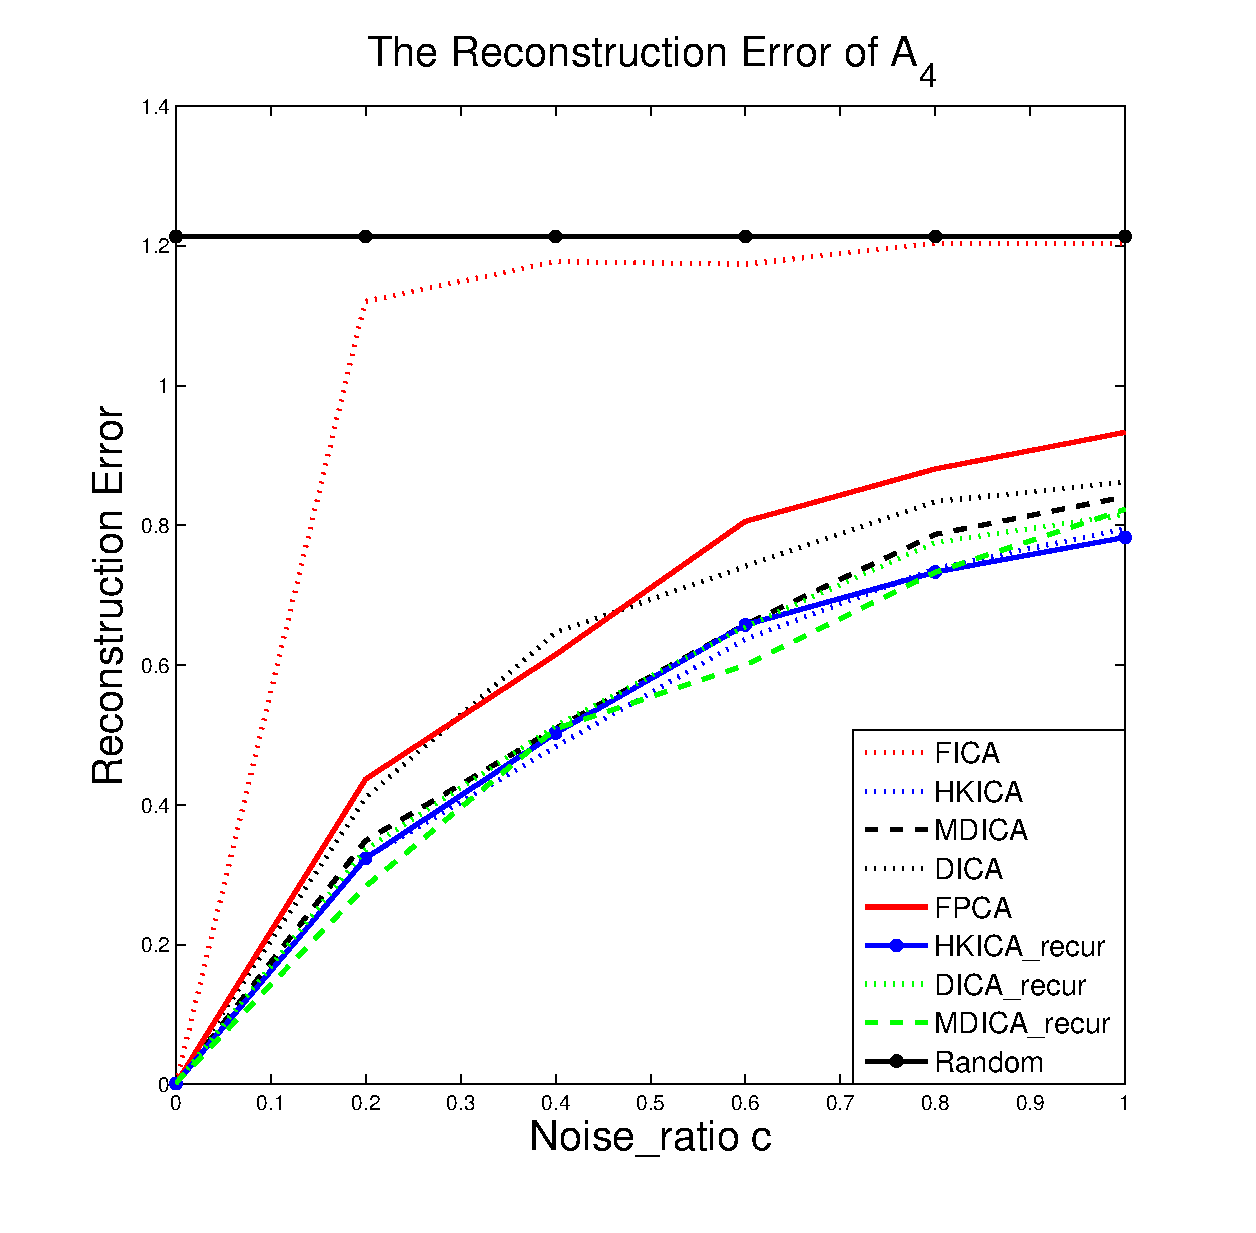
\includegraphics[width =0.45\columnwidth]{error4_d3}
\caption{
\label{fig:Error_d3}
 Reconstruction Errors: Dimension 3; X axis: noise ratio; Sample size: 20000.}
\end{figure}

\section{Experimental Results of different sample sizes}
\subsection{noise-free case}
The reconstruction errors for different sample sizes in a noise-free setting are as follows. 
\begin{figure}[t] %pt]
	\includegraphics[width =0.45\columnwidth]{errorR_sample_noise0}
	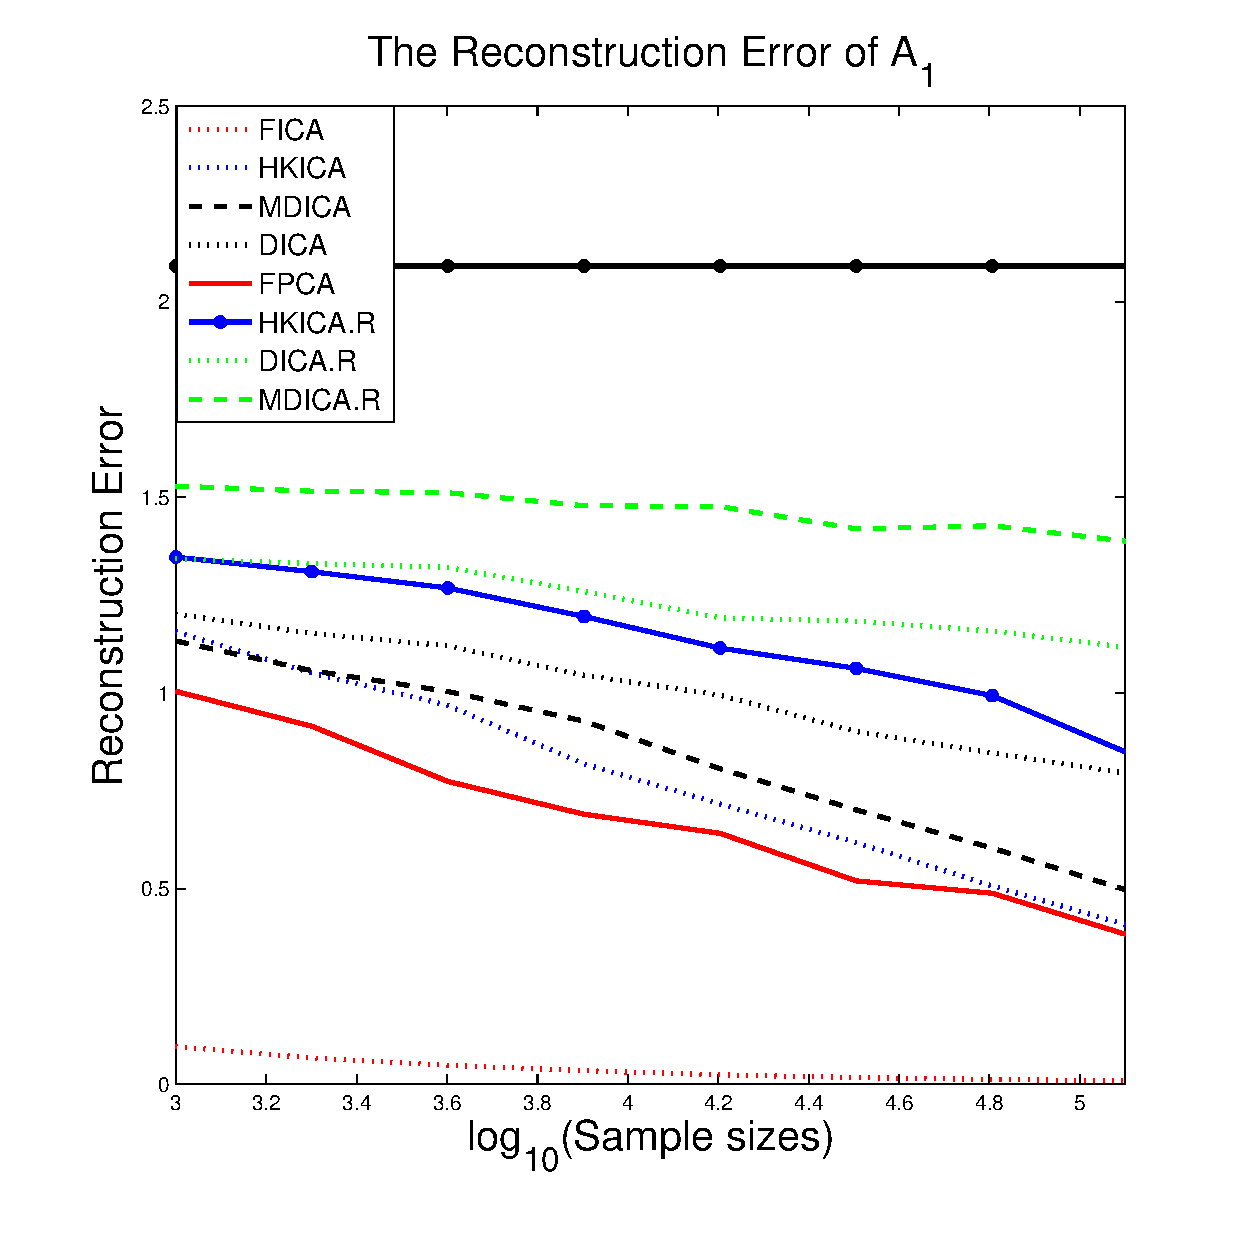
\includegraphics[width =0.45\columnwidth]{error1_sample_noise0} \\
	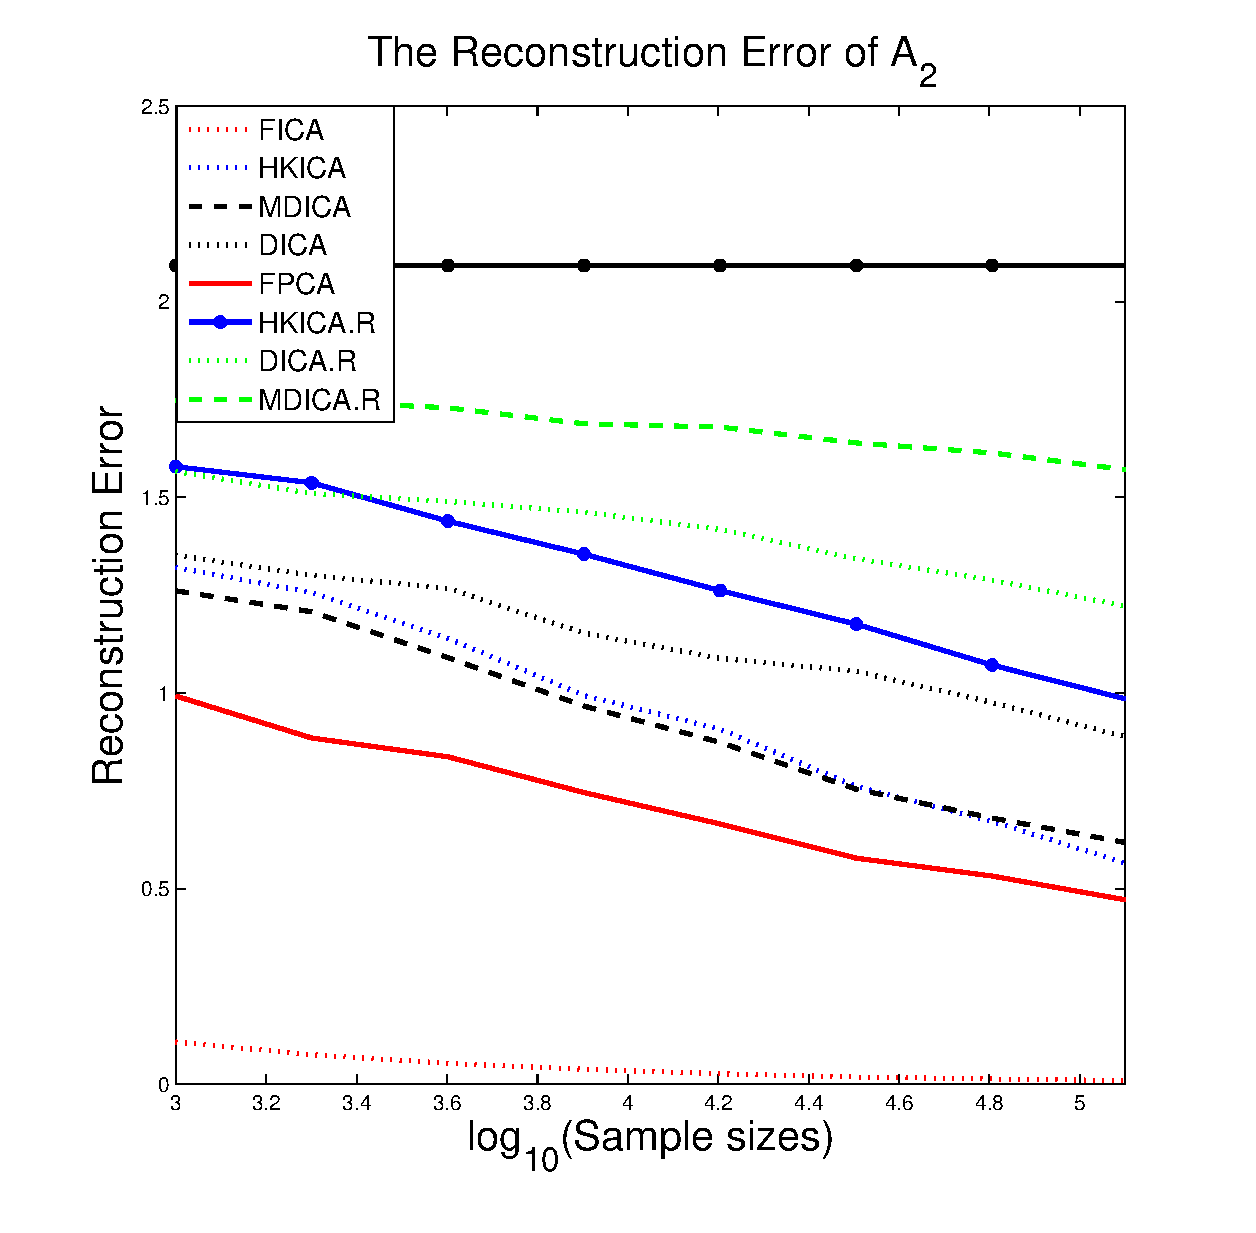
\includegraphics[width =0.45\columnwidth]{error2_sample_noise0}
	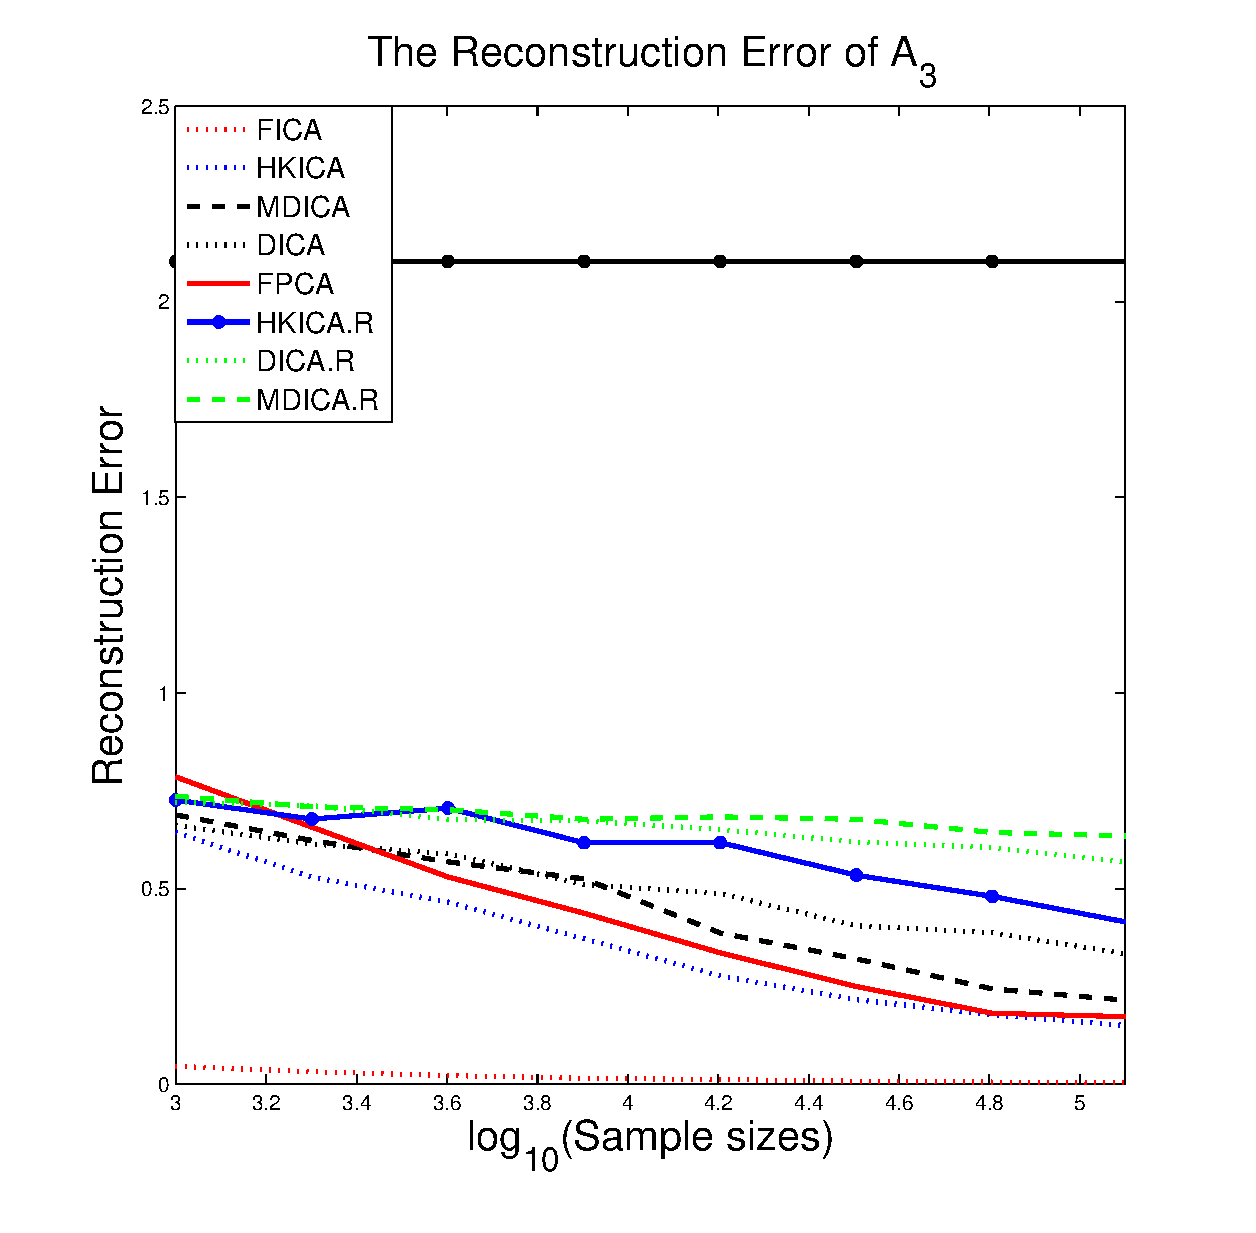
\includegraphics[width =0.45\columnwidth]{error3_sample_noise0} \\
	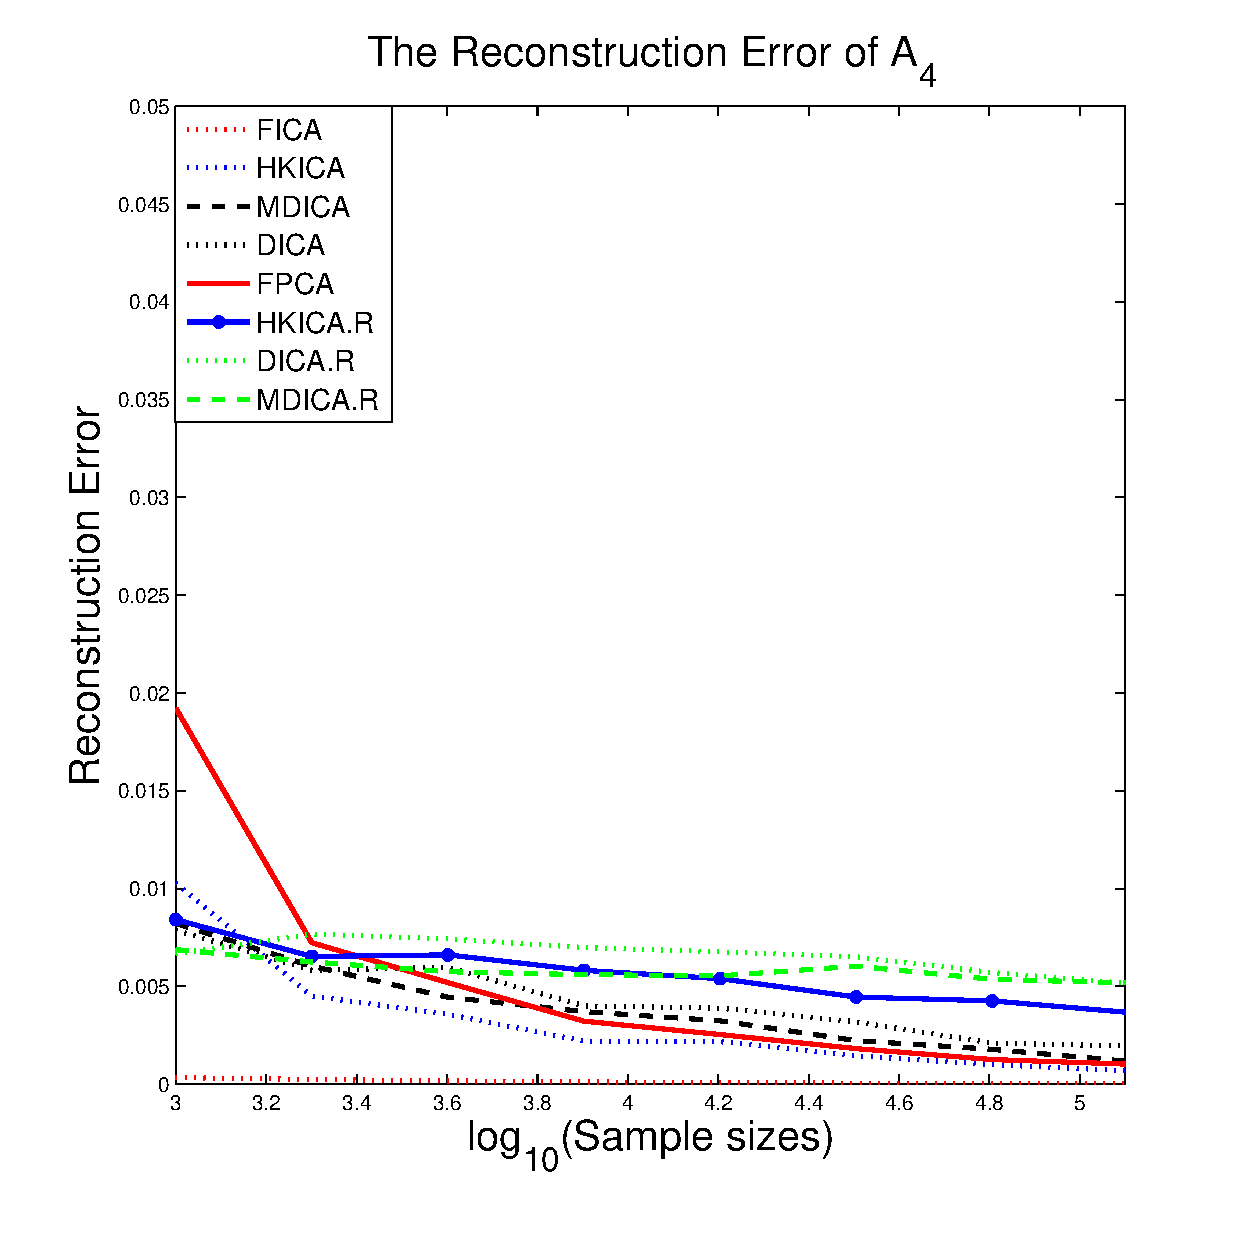
\includegraphics[width =0.45\columnwidth]{error4_sample_noise0}
\caption{
\label{fig:Error_sample_noise0}
 Reconstruction Errors: Dimension 6; X axis: sample size; Noise ratio: 0.}
\end{figure}

\subsection{the case of noise ratio 0.3}
The reconstruction errors for different sample sizes in a noise-free setting are as follows. 
\begin{figure}[t] %pt]
	\includegraphics[width =0.45\columnwidth]{errorR_sample_noise3}
	\includegraphics[width =0.45\columnwidth]{error1_sample_noise3} \\
	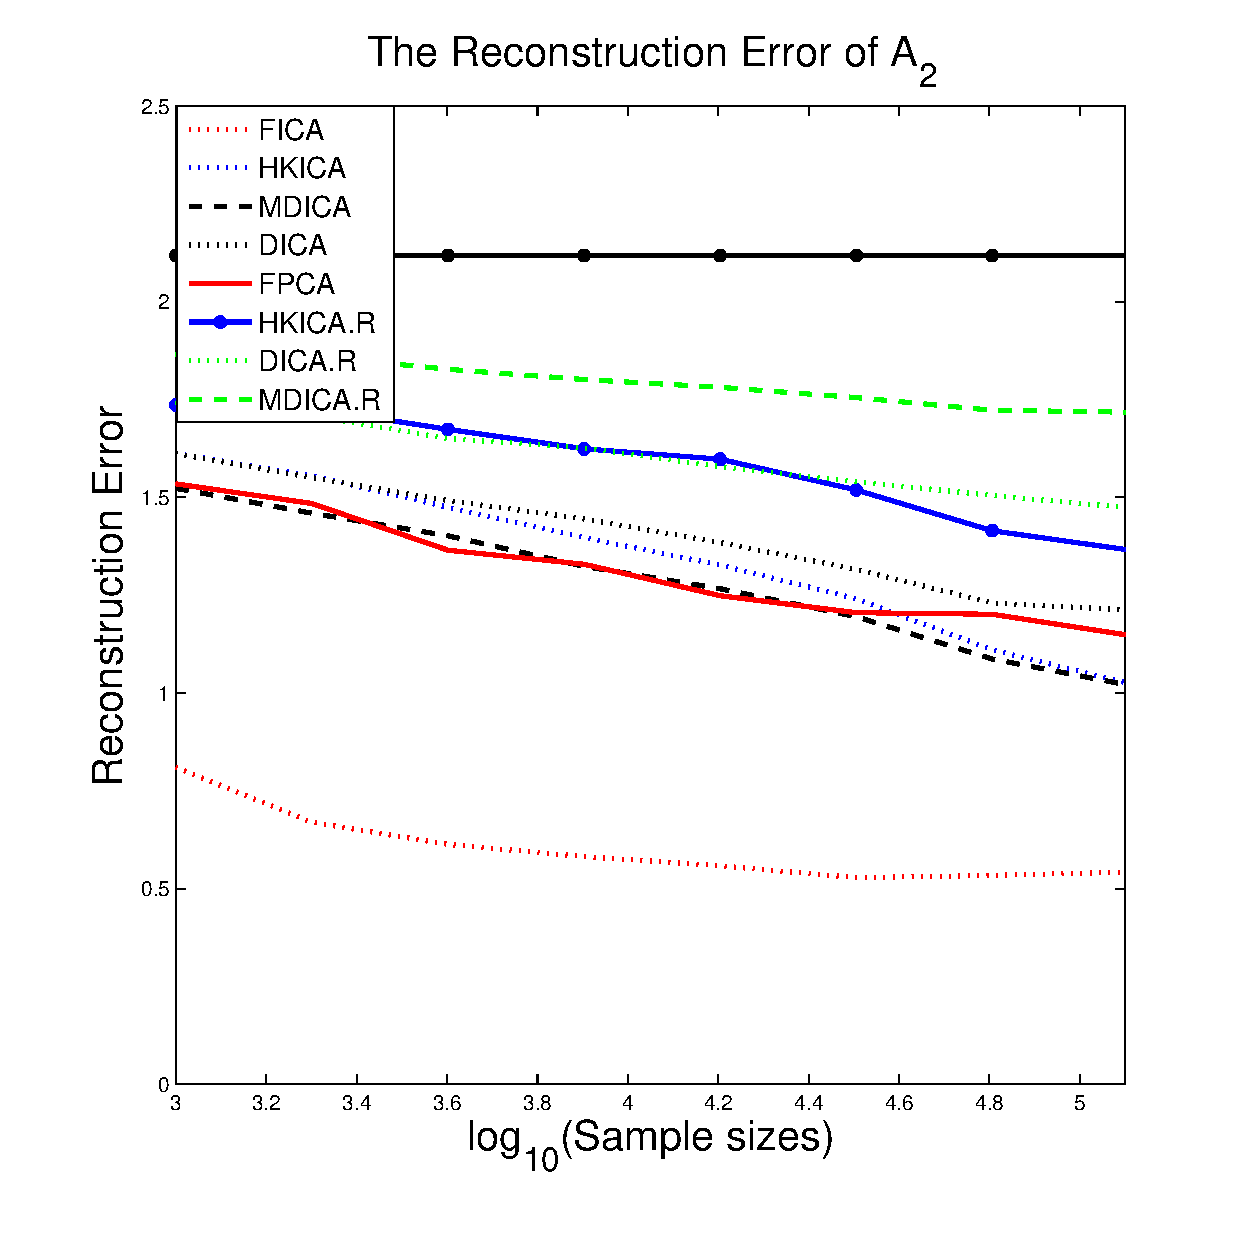
\includegraphics[width =0.45\columnwidth]{error2_sample_noise3}
	\includegraphics[width =0.45\columnwidth]{error3_sample_noise3} \\
	\includegraphics[width =0.45\columnwidth]{error4_sample_noise3}
\caption{
\label{fig:Error_sample_noise3}
 Reconstruction Errors: Dimension 6; X axis: sample size; Noise ratio: 0.3.}
\end{figure}

\subsection{the case of noise ratio 0.3}
The reconstruction errors for different sample sizes in a noise-free setting are as follows. 
\begin{figure}[t] %pt]
	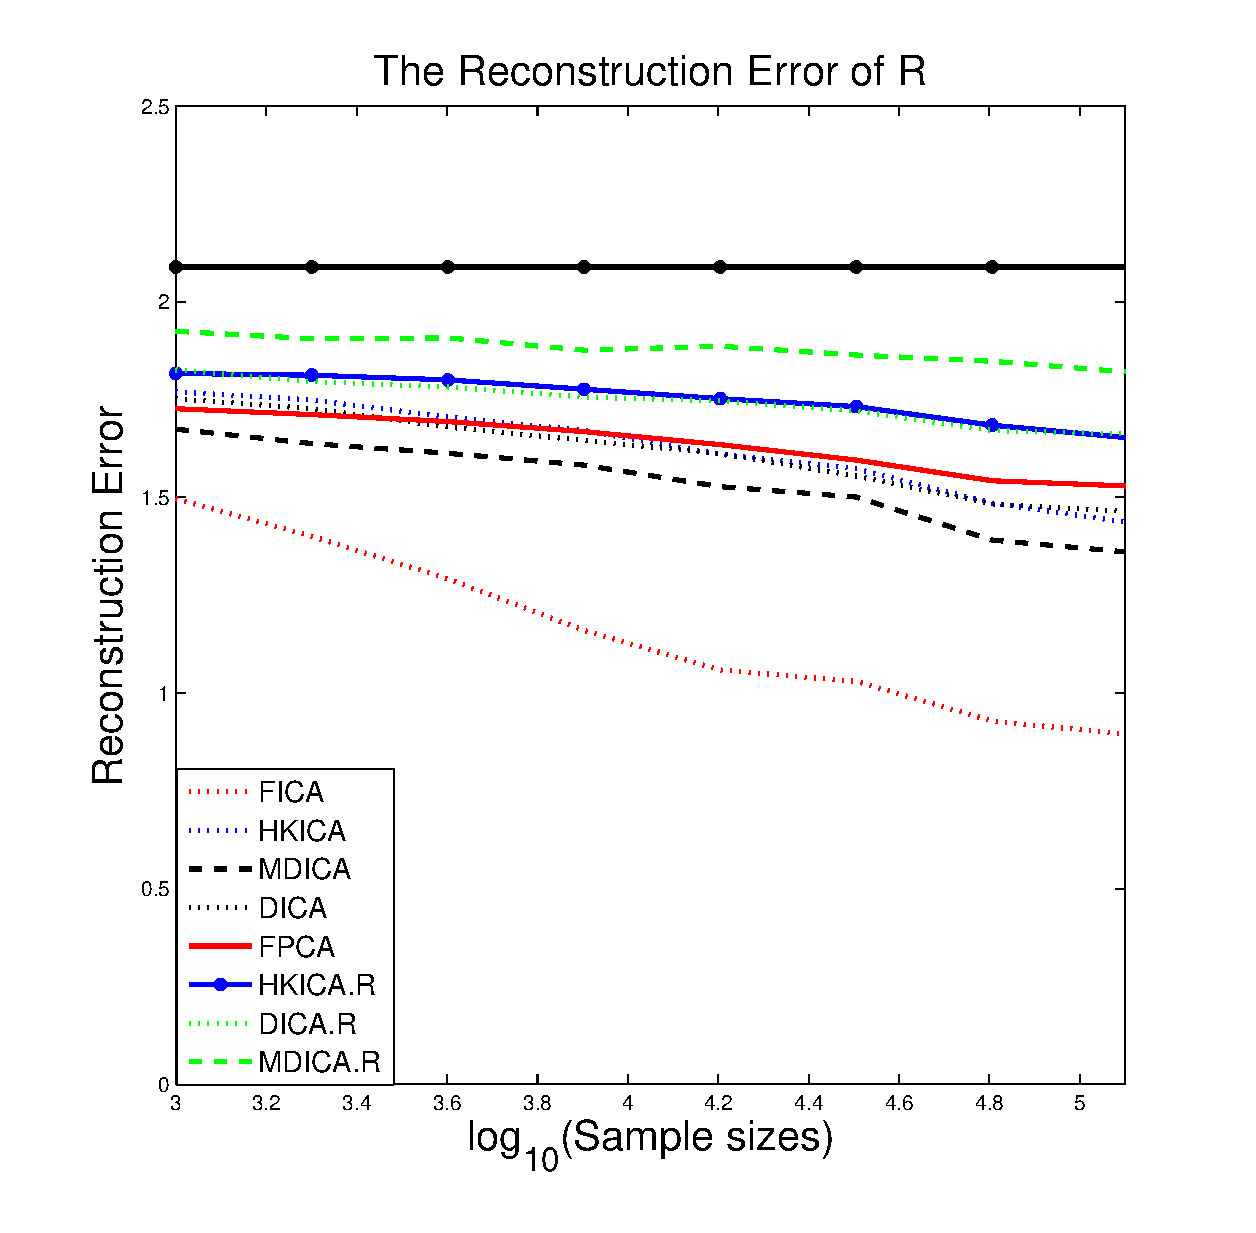
\includegraphics[width =0.45\columnwidth]{errorR_sample_noise6}
	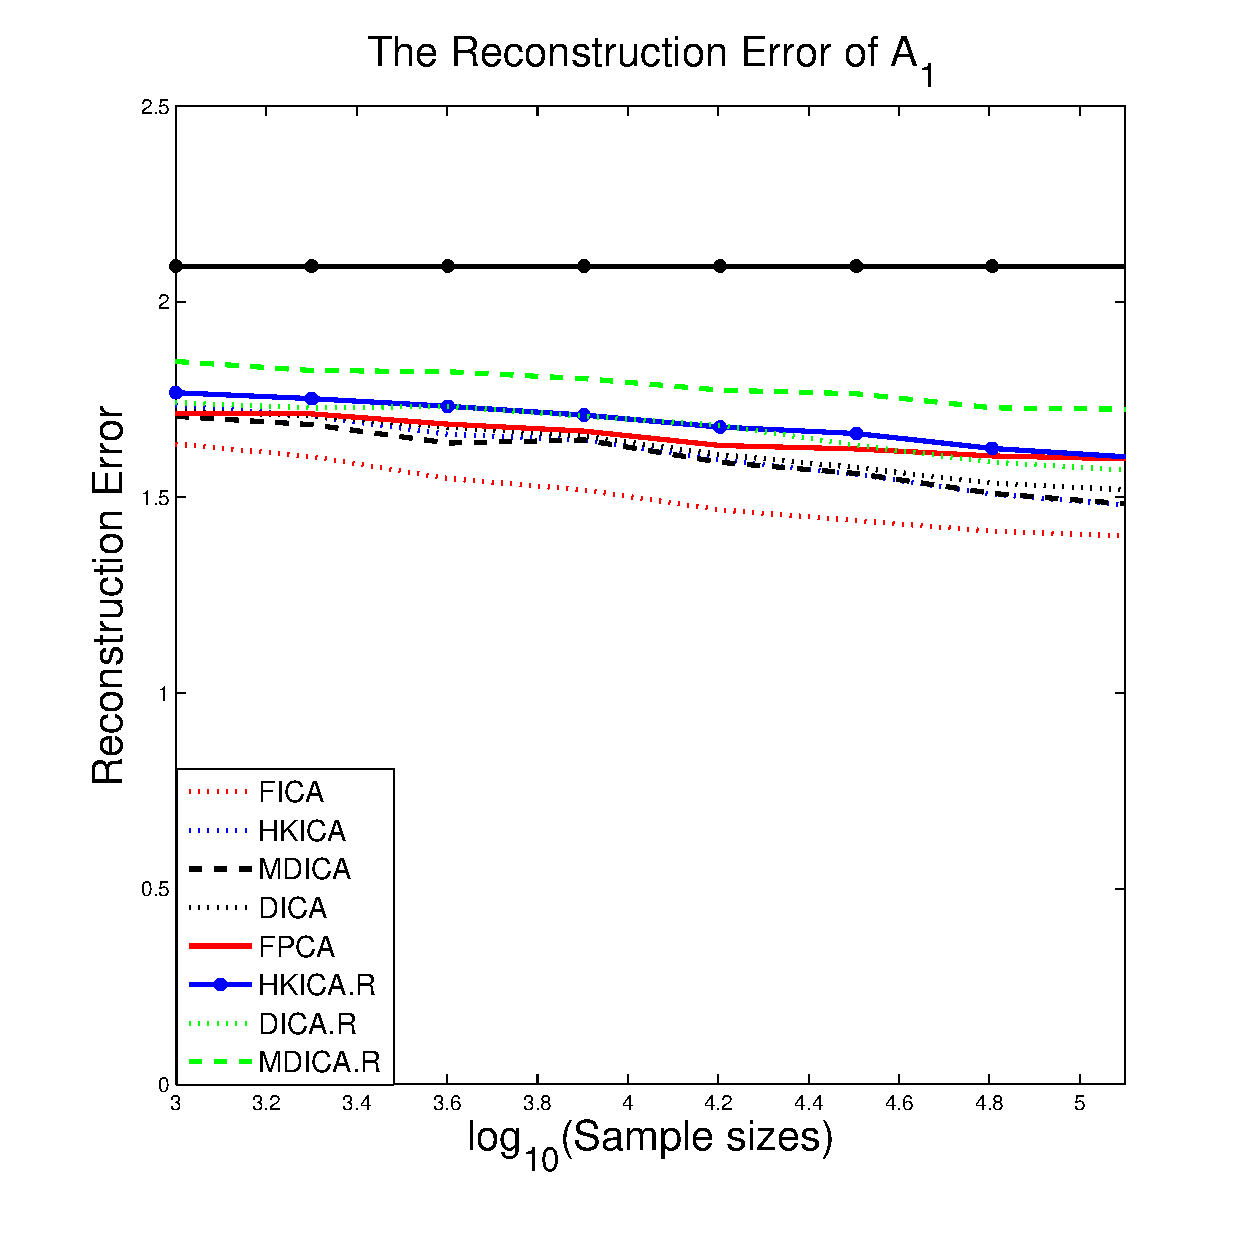
\includegraphics[width =0.45\columnwidth]{error1_sample_noise6} \\
	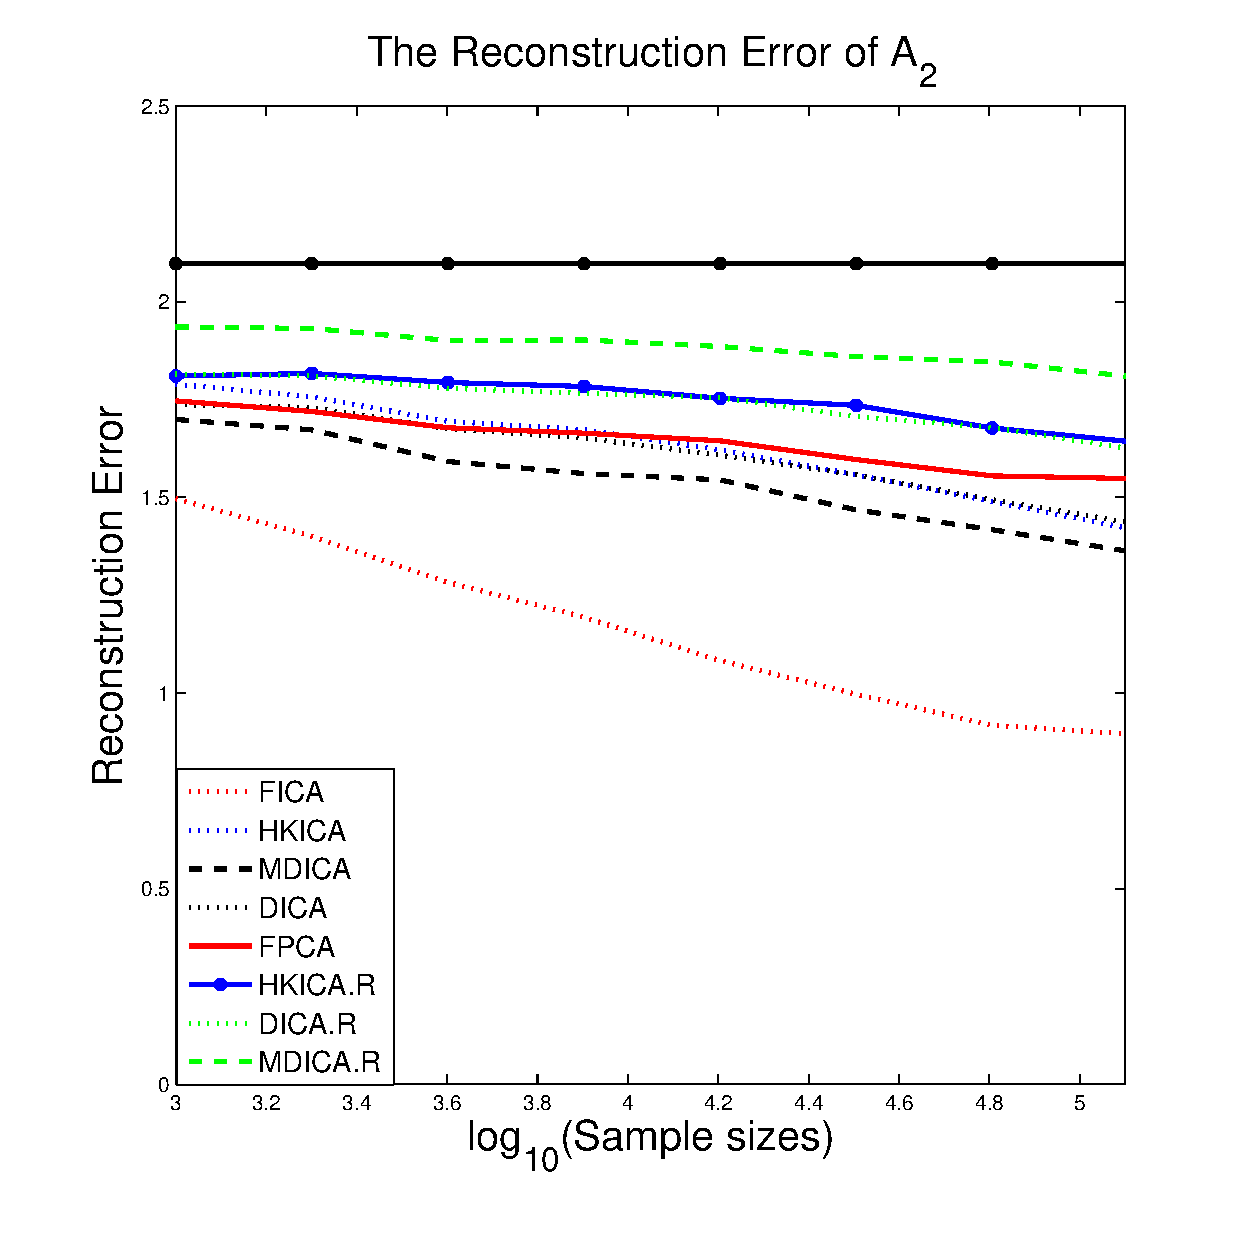
\includegraphics[width =0.45\columnwidth]{error2_sample_noise6}
	\includegraphics[width =0.45\columnwidth]{error3_sample_noise6} \\
	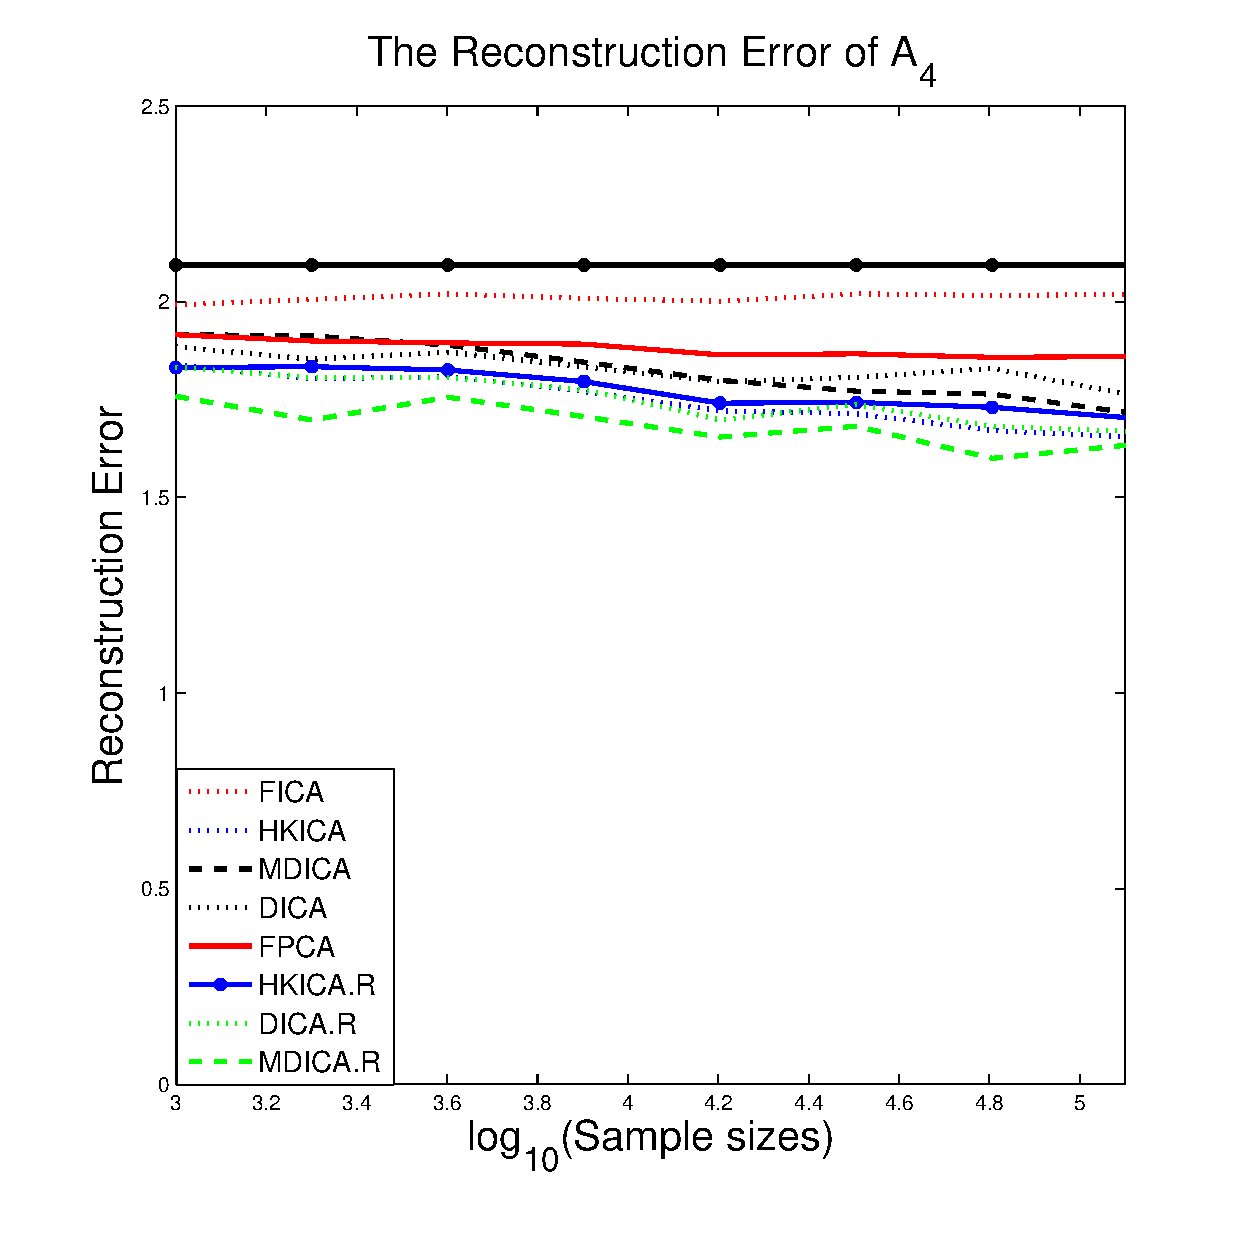
\includegraphics[width =0.45\columnwidth]{error4_sample_noise6}
\caption{
\label{fig:Error_sample_noise6}
 Reconstruction Errors: Dimension 6; X axis: sample size; Noise ratio: 0.6.}
\end{figure}


%%% Local Variables: 
%%% mode: latex
%%% TeX-master: "DICA"
%%% End: 
